\documentclass[border=6pt]{standalone}
% Shared typography and colours for the standalone figures.
\usepackage{unicode-math}
\setmainfont{TeX Gyre Heros}
\setmathfont{TeX Gyre Pagella Math}
\usepackage{tikz}
\usetikzlibrary{arrows.meta,positioning,calc,decorations.pathreplacing}
\usepackage{pgfplots}
\pgfplotsset{compat=1.18}

% One colour per element or subsystem. Record the mapping in
% the working repository conventions and use it identically in every figure.
\definecolor{elemA}{HTML}{1F5FA8}
\definecolor{elemB}{HTML}{B8461B}
\definecolor{elemC}{HTML}{2E7D32}
\definecolor{elemD}{HTML}{6A4C93}
\definecolor{frameline}{HTML}{555555}

\begin{document}
\hyphenpenalty=10000
\exhyphenpenalty=10000
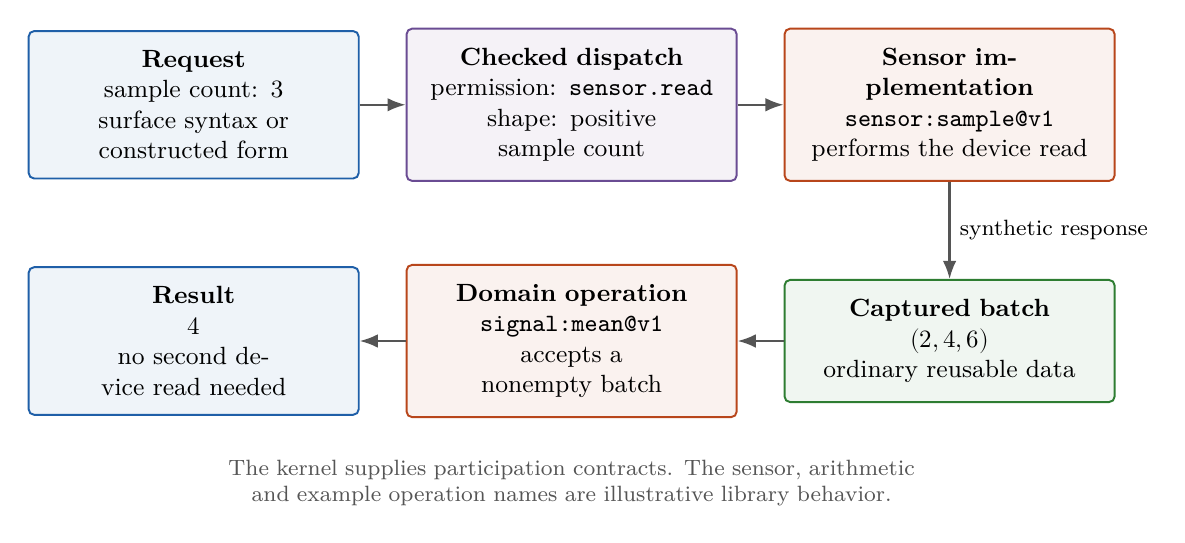
\begin{tikzpicture}[font=\small,
box/.style={draw=#1,fill=#1!7,rounded corners=2pt,line width=.7pt,text width=3.7cm,minimum height=1.45cm,align=center,inner sep=7pt},
arrow/.style={-{Latex[length=2.3mm]},line width=.8pt,draw=frameline}]
\node[box=elemA] (request) at (-4.8,2.8) {\textbf{Request}\\sample count: 3\\surface syntax or constructed form};
\node[box=elemD] (checks) at (0,2.8) {\textbf{Checked dispatch}\\permission: \texttt{sensor.read}\\shape: positive sample count};
\node[box=elemB] (sensor) at (4.8,2.8) {\textbf{Sensor implementation}\\\texttt{sensor:sample@v1}\\performs the device read};
\draw[arrow] (request)--(checks);
\draw[arrow] (checks)--(sensor);
\node[box=elemC] (batch) at (4.8,-.2) {\textbf{Captured batch}\\$(2,4,6)$\\ordinary reusable data};
\node[box=elemB] (mean) at (0,-.2) {\textbf{Domain operation}\\\texttt{signal:mean@v1}\\accepts a nonempty batch};
\node[box=elemA] (result) at (-4.8,-.2) {\textbf{Result}\\$4$\\no second device read needed};
\draw[arrow] (sensor)--node[right,font=\footnotesize]{synthetic response}(batch);
\draw[arrow] (batch)--(mean);
\draw[arrow] (mean)--(result);
\node[align=center,text width=13cm,font=\footnotesize,text=frameline] at (0,-2)
 {The kernel supplies participation contracts. The sensor, arithmetic and example operation names are illustrative library behavior.};
\end{tikzpicture}
\end{document}
